%%=================================================================%%
%% Author : P�rez Ruiz, Alejandro                                  %%
%% Author : S�nchez Barreiro. Pablo                                %%
%%                                                                 %%
%% Version: 1.0, 16/03/2011                                        %%                                                                                    %% Version: 1.1, 20/06/2011                                        %%                                                                                    %%                                                                 %%
%%                                                                 %%
%% Memoria del Proyecto Fin de Carrera                             %%
%% ApplicationEngineering/DSL                                      %%  
%%=================================================================%%


La idea que subyace detr�s de la automatizaci�n del desarrollo software dirigida por modelos~\cite{} es crear alg�n tipo de lenguaje de modelado que permita especificar productos concretos. Estos lenguajes reciben el nombre de \emph{lenguajes espec�ficos de dominio} (\emph{DSL}, por sus siglas en ingl�s \emph{Domain Specific Language})~\cite{kleppe:2008} . Dichos lenguajes deber�an ser tan simples y f�ciles de usar como fuese posible, permitiendo que incluso usuarios finales, no necesariamente relacionados con el mundo del desarrollo software pero si familiares con el dominio, pudiesen especificar ellos mismo que productos concretos desean obtener de nuestra l�nea de productos. A continuaci�n, el c�digo necesario para componer e instanciar las caracter�sticas seleccionadas se generar�a de forma autom�tica a partir de un modelo de un producto concreto.

Para definir un lenguaje espec�fico de dominio, el primer paso a realizar es definir su sintaxis abstracta o gram�tica, lo cual se realiza mediante la construcci�n de un metamodelo~\cite{kleppe:2008} para dicho DSL. Un metamodelo se puede definir de manera informal como un modelo de la sintaxis de todos los modelos que se pueden construir usando el DSL que especifica. El metamodelo para una l�nea de productos deber�a procurar, que en la medida de lo posible, evitar que se puedan crear configuraciones que den lugar a productos err�neos o no seguros. Por ejemplo, en nuestro caso, el propio metamodelo deber�a evitar que se puedan crear productos que contengan funcionalidades para el control inteligente de a energ�a para una casa que no tenga ning�n aparato de control de la temperatura automatizado. 

Para crear dicho metamodelo, hacemos uso de la herramienta que proporciona el entorno de desarrollo Visual Studio 2010 para tal fin: \emph{Domain-Specific Language Tools (DSL Tools)}~\cite{jones:2011}. Las DSL Tools proporcionan  facilidades para crear un metamodelo, generar autom�ticamente un editor que permitan crear modelos visuales conformes a dicho metamodelo as� como crear generadores de c�digo para los modelos producidos con dicho editor.

\begin{figure}[!tb]
 \centering
 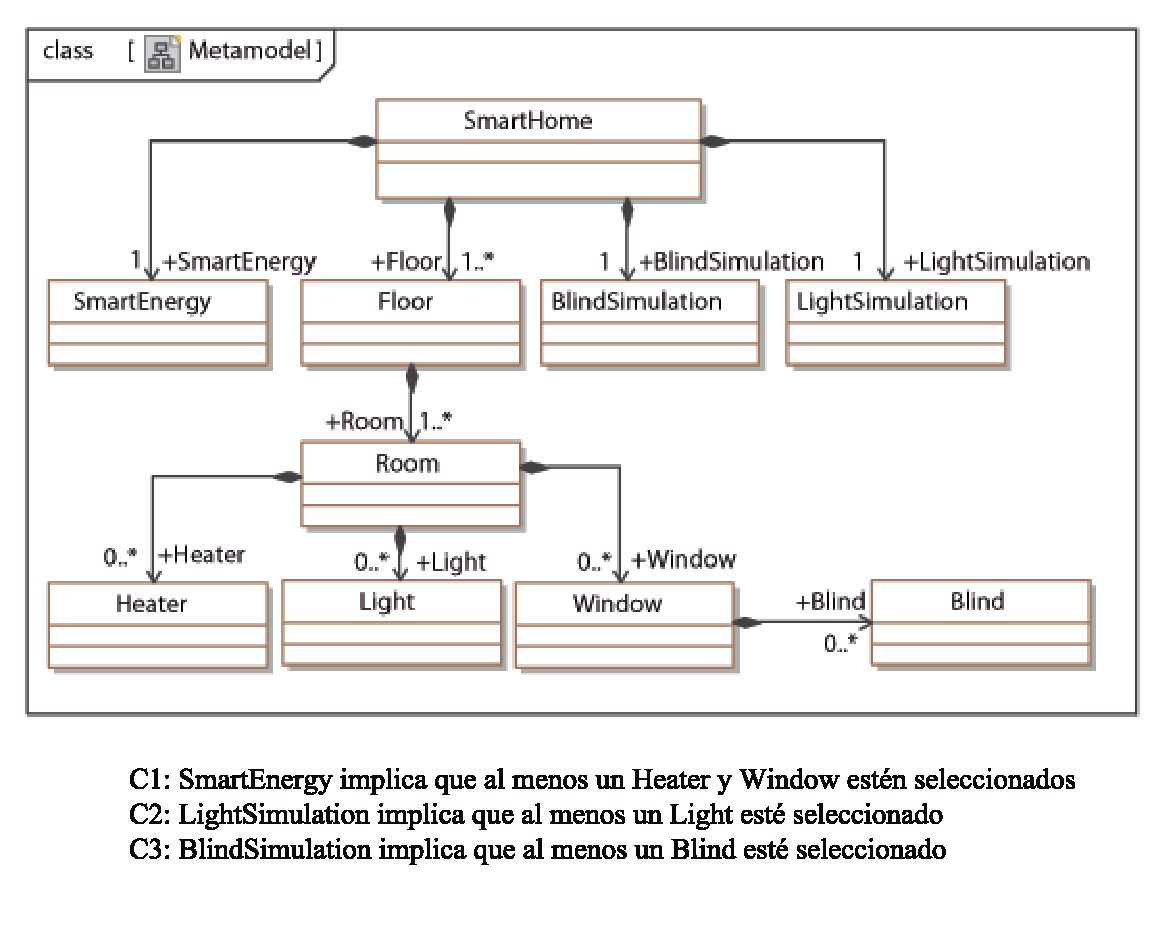
\includegraphics[width=.65\linewidth]{applicationEngineering/images/metaModel.eps} \\
 \caption{Metamodelo para un hogar inteligente}
 \label{app:fig:metamodel}
\end{figure}

La Figura~\ref{app:fig:metamodel} muestra el metamodelo creado para la configuraci�n de productos concretos dentro de nuestra l�nea de productos. Un metamodelo se describe normalmente usando una versi�n compacto de los diagramas de clases de UML\footnote{En realidad, la notaci�n es similar a la de los diagramas de clases UML, pero corresponde al lenguaje de metamodelado MOF}. En nuestra caso, el metamodelo muestra por ejemplo que ...

%%=================================================================%%
%% NOTA(Pablo): Describe aqu� algo del metamodelo para que se vea  %%
%%              como funciona                                      %%
%%=================================================================%%

No obstante, no todas las restricciones existentes en un cierto dominio pueden modelarse usando la notaci�n propia de los diagramas de clase UML, por lo que a veces es necesario definir ciertas restricciones externas, usando lenguajes como OCL~\cite{}. En nuestro caso, se definen tres restricciones, las cuales aparecen en la parte baja de la Figura~\ref{app:fig:metamodel}. En nuestro caso, el editor generado autom�ticamente a partir de este metamodelo se enriquece con una serie de funciones destinadas a comprobar que dichas restricciones no se violan cuando se crean productos concretos. De esta forma, los modelos creados y validados por el editor siempre representar�n productos correctos, siendo una entrada v�lida para los generadores de c�digo.

%%=================================================================%%
%% NOTA(Pablo): Estas 3 restricciones est�n mal definidas. O usas  %%
%%              OCL o en texto                                     %%   
%%=================================================================%%
 
De esta forma se consigue integrar en el propio entorno de Visual Studio 2010 una nueva herramienta que permite construir modelos espec�ficos que representan productos concretos. Adem�s, se comprueba que dichas configuraciones no sean incorrectas. La siguiente secci�n describe como construir un generador de c�digo que autom�ticamente componga e instancie caracter�sticas de acuerdo al esquema especificado en la secci�n anterior.


